\section{PyTorch Fuzzing}

PyTorch is a popular open-source machine-learning framework that has gained immense popularity in recent years. Developed by Meta (formerly Facebook), PyTorch has emerged as one of the most widely used machine learning frameworks due to its ease of use, flexibility, and dynamic computational graph, making it a popular choice for researchers and developers alike.

PyTorch is a critical component of many applications across various industries such as banking, healthcare, insurance, and many others. It is used for natural language processing, image classification, speech recognition, and other tasks. In banking, PyTorch is used to develop fraud detection systems, while in healthcare, it is used to diagnose diseases and predict patient outcomes. The insurance industry uses PyTorch to analyze risk and predict losses. The flexibility of PyTorch enables it to be used in many other domains as well. PyTorch has been used to build many state-of-the-art machine learning models and is a vital tool in the field of deep learning.

Despite its popularity and usefulness, PyTorch has several challenges that must be addressed to ensure its reliability and security. PyTorch has multiple dependencies, and it includes a considerable amount of C/C++ code which implies that it is susceptible to memory safety vulnerabilities. Moreover, PyTorch is an interesting target for adversaries since it is used in critical applications. Therefore, it is crucial to ensure that PyTorch is secure and free from vulnerabilities. Fuzzing is a valuable technique that can help identify bugs and vulnerabilities in PyTorch, making it more robust and secure. By fuzzing PyTorch, we can ensure that it can withstand attacks and continue to operate correctly in real-world applications.

In this chapter, we will explore the concept of PyTorch fuzzing and its significance in improving the reliability and security of PyTorch. We will begin by describing its attack surface. We will then develop fuzzing harnesses for the interesting parts of the codebase. Finally, we will describe the fuzzing methodology and the results of our work.

\subsection{Attack Surface Mapping}

To begin our fuzzing efforts, we must first identify the attack surface of PyTorch. The attack surface refers to all the entry points through which an attacker can potentially interact with the system and launch an attack. In the case of PyTorch, its attack surface includes various modules, libraries, and dependencies that it uses.

To identify interesting parts of the codebase that are relevant to the attack surface, we have performed manual code analysis. Our analysis has highlighted several modules that are particularly interesting to fuzz, including the model loading and RPC communications modules.

\subsubsection{Model Loading}

The process of loading pre-trained models is a crucial entry point that attackers can exploit to gain access to the system. This process is typically handled by the model loading module, which can be accessed via the \texttt{torch.load()} function.

During the loading process, the \texttt{torch.load()} function goes through several deserialization steps, also known as unpickling, to recreate the original object from the byte stream. Deserialization is a common source of vulnerabilities in many applications, as it can be difficult to implement correctly. Unfortunately, PyTorch is not immune to this issue. Additionally, since the implementation is written in C++, it is even more susceptible to memory safety vulnerabilities.

The code responsible for model loading and parsing is mostly located in these files:

\begingroup
\begin{itemize}
    \item jit/serialization/import.cpp
    \item jit/ir/irparser.cpp
    \item jit/serialization/unpickler.cpp
    \item jit/runtime/interpreter.cpp
    \item jit/frontend/schema\_type\_parser.cpp
\end{itemize}
\endgroup

\subsubsection{Remote Communications (RPC)}

Besides model loading, PyTorch has another interesting mechanism that attackers can exploit - the RPC communications module.

The RPC module in PyTorch is a complex system that opens up new, remotely accessible attack vectors. PyTorch uses the RPC module to implement distributed training and inference that allows users to train and execute models across multiple machines. This feature is essential for large-scale applications that require high computational power. However, it increases the security risks by creating additional entry points for attackers.

PyTorch uses various types of RPCs such as \texttt{RRef} (Remote Reference),\\ \texttt{ScriptCall}, and others to interact with remote machines. Before sending RPCs, they are serialized into pickled objects using the \texttt{torch::jit::pickle} function. The RPCs are then sent using different backends like TensorPipe, Gloo, and MPI. Once received, the RPCs are deserialized using the \texttt{torch::jit::unpickle} function, and the target \texttt{Message}'s class \texttt{fromMessage()} method is called. This leaves the receiver with a plain message that can be further processed.

Unfortunately, the complexity of this system makes it prone to bugs and vulnerabilities. Multiple serializations and deserializations of messages can introduce bugs, and the fact that the RPC protocol is implemented in C++ makes it an attractive target to look for memory safety vulnerabilities. Moreover, given the memory-unsafe nature of the RPC protocol, a single bug could potentially allow an attacker to execute code remotely on a target machine. As a result, fuzzing the RPC module is highly recommended to identify and address potential vulnerabilities.

With that in mind, we have identified the following files as the most interesting targets for security research:

\begingroup
\begin{itemize}
    \item distributed/rpc/*.cpp
    \item jit/serialization/unpickler.cpp
\end{itemize}
\endgroup

\subsubsection{Finding Fuzz-Targets}

Now that we have identified different parts of the PyTorch codebase that are relevant to the attack surface, we can proceed to the second part of the attack surface mapping - identifying specific functions and methods to fuzz.

To achieve this, we have used two different approaches:

\begin{enumerate}
    \item \textbf{Manual code review} - we have performed a manual code review of the PyTorch codebase to identify relevant functions that are confined to the defined attack surface.
    \item \textbf{CodeQL} - we have used CodeQL \cite{ql-object-oriented-queries-on-relational-data} to broadly search for interesting functions and methods that perform some kind of deserialization or parsing.
\end{enumerate}

The first approach is straightforward and does not require any additional tools. However, it is time-consuming and requires a lot of manual work. Nevertheless, it yields the best results since it allows us to precisely identify the functions that might be interesting to fuzz.

The second approach lacks "precision" but can be automated and scaled to a large codebase. It allows us to quickly identify a narrowed-down set of functions that are worth looking into. However, it is not as precise as the first approach since it relies on heuristics and does not "understand" the code. As a result, it can miss some relevant functions. Nevertheless, it is a good starting point for fuzzing since it can help identify interesting functions that can be further analyzed manually.

To begin with, we employed the second approach to pinpoint some specific functions that are worth looking into. We developed a CodeQL query \ref{appendix:codeql-query} that searches for functions that have two parameters:

\begin{enumerate}
    \item The first parameter is a pointer to data of "parsable" types. For example - \texttt{char*}, \texttt{byte*}, and others.
    \item The second parameter is an integer that represents the size of the data. For example - \texttt{int}, \texttt{size\_t}, and others.
\end{enumerate}

With that in place, we added a few more heuristics to filter out irrelevant functions. Finally, we used \textit{Cyclomatic Complexity} \cite{cyclomatic-complexity-density} to rank the results and identify the most complex functions. Some results of the query are shown in Table \ref{table:codeql-results}.

\begin{table}[h]
    \centering
    \begin{tabular}{cl}
        \toprule
        \textbf{Complexity} & \textbf{Function}                      \\
        13                  & \texttt{rpc::parseWireSections}        \\
        6                   & \texttt{Unpickler::readSlowWithBuffer} \\
        5                   & \texttt{TokenTrie::insert}             \\
        4                   & \texttt{rpc::wireDeserialize}          \\
        \bottomrule
    \end{tabular}
    \caption{CodeQL query results}
    \label{table:codeql-results}
\end{table}

These results gave us a good starting point. From here, we manually reviewed the functions and started to study the codebase, employing the first approach.

Finally, we have compiled a list of the most interesting functions that are worth fuzzing. The list is shown in Table \ref{table:fuzz-targets}.

\begin{table}[h]
    \centering
    \begin{tabular}{cl}
        \toprule
        \textbf{Function}                 \\
        \texttt{jit::parseIR}             \\
        \texttt{jit::load}                \\
        \texttt{rpc::deserializeResponse} \\
        \texttt{rpc::deserializeRequest}  \\
        \bottomrule
    \end{tabular}
    \caption{Fuzz targets}
    \label{table:fuzz-targets}
\end{table}

The first two functions are related to the JIT module and are responsible for parsing and loading the pickled data. Some examples of such data are: \texttt{saved models}, \texttt{serialized request}, and others.

The last two functions are related to the RPC module and are responsible for deserializing RPC requests and responses. These functions are interesting because they are directly processing untrusted data that is received from the network.

Besides that, we have also identified another interesting function - \\ \texttt{jit::preoptimizeGraph}, which is a part of the JIT module. We decided to target it with differential fuzzing to find bugs related to the optimization of the JIT graphs.

\subsection{Preparing PyTorch for Fuzzing}
\subsubsection{Fuzzing Harness Development}

With the fuzz targets identified, we can proceed to the next step - developing a fuzzing harness. The goal of the fuzzing harness is to provide a way to feed the fuzz target with data and collect the results of the execution. For our purposes, we have developed a \textit{LibFuzzer}-compatible \cite{libfuzzer-secdev-2016} targets for each of the functions listed in Table \ref{table:fuzz-targets}.

Each libFuzzer-based target shares the same structure. The structure is shown in Listing \ref{listing:fuzz-target-structure}.

\begin{listing}[h]
    \centering
    \begin{minipage}{.9\linewidth}
        \begin{minted}[linenos=true, tabsize=4]{cpp}
int LLVMFuzzerTestOneInput(const uint8_t* data, size_t size) {
    // 1. Parse the input data
    // 2. Call the fuzz target with the parsed data
    // 3. Return 0
}
    \end{minted}
    \end{minipage}
    \caption{Fuzz target structure}
    \label{listing:fuzz-target-structure}
\end{listing}

The goal of a generic fuzzing harness is to pass the data generated by the fuzzer to the fuzz target and clean up the resources after the execution is finished. The fuzzing harness is also responsible for handling the exceptions that might be thrown by the fuzz target.

The fuzzing harnesses that we have developed for PyTorch are similar to the generic one. However, they also perform some additional steps. For example, they handle some PyTorch-specific exceptions.

The developed fuzzing harnesses are listed below:

\begin{itemize}
    \item \href{https://github.com/ispras/oss-sydr-fuzz/blob/028e36875424aec00ef7375006c413a4be164197/projects/pytorch/irparser_fuzz.cc}{\texttt{irparser\_fuzz.cc}} - fuzzes \texttt{jit::parseIR}
    \item \href{https://github.com/ispras/oss-sydr-fuzz/blob/028e36875424aec00ef7375006c413a4be164197/projects/pytorch/load_fuzz.cc}{\texttt{load\_fuzz.cc}} - fuzzes \texttt{jit::load}
    \item \href{https://github.com/ispras/oss-sydr-fuzz/blob/028e36875424aec00ef7375006c413a4be164197/projects/pytorch/message_deserialize_fuzz.cc}{\texttt{message\_deserialize\_fuzz.cc}} - fuzzes \texttt{rpc::deserializeResponse} and \texttt{rpc::deserializeRequest}
    \item \href{https://github.com/ispras/oss-sydr-fuzz/blob/028e36875424aec00ef7375006c413a4be164197/projects/pytorch/jit_differential_fuzz.cc}{\texttt{jit\_differential\_fuzz.cc}} - fuzzes three related methods - \texttt{jit::parseIR}, \texttt{jit::preoptimizeGraph}, and \texttt{jit::InterpreterState(code).run()} with differential fuzzing
\end{itemize}

However, the development of fuzzing harnesses is only another step toward hybrid fuzzing. The next step is to compile all the necessary build targets and prepare the environment.

\subsubsection{Build Targets Compilation}

To meet the requirements of hybrid fuzzing, we need to compile a few different types of build targets.

The first one is the fuzz target itself. It is the main entry point for the fuzzer. This target is compiled using the \textit{clang} compiler with the \textit{libFuzzer} library linked. To achieve this, we have added the following compilation flags to the build script: \texttt{-fPIC -g -fsanitize=fuzzer,address,bounds}. To easily distinguish the fuzz target from other targets, we have also added the \texttt{\_fuzz} suffix to the name of the produced binary.

The second type of build target is the plain binary, which reads the data directly from the file and passes it to the fuzz target, without involving the fuzzer. It allows the symbolic execution engine to execute the fuzz target with concrete data. This target is also compiled with the help \textit{clang} compiler, however, the flags are different: \texttt{-fPIC -g}. We have also added the \texttt{\_sydr} suffix to the name of the binary.

And the last type of build target is the binary that is used to collect the coverage information. It is compiled with the \textit{clang} compiler and the following flags: \texttt{-fPIC -g -fprofile-instr-generate -fcoverage-mapping}. As for the previous targets, we have also added the \texttt{\_cov} suffix to the name of the binary.

\subsection{PyTorch Hybrid Fuzzing}

With all the artifacts produced, we can now proceed to the next step - hybrid fuzzing. The goal of this step is to prepare the environment, perform the fuzzing, and analyze the results. To perform hybrid fuzzing, we have used the \textit{sydr-fuzz}, a tool developed by ISP RAS. \textit{Sydr-fuzz} is a flexible framework for hybrid fuzzing, which allows us to easily perform the fuzzing of the target program with the help of the symbolic execution engine and state-of-the-art fuzzers such as \textit{AFL++} and \textit{libFuzzer}.

\subsubsection{Preparing the Environment}

Before we can start the fuzzing, we need to prepare the environment. The preparation includes many steps, however, in our case, we only need to perform a single step - to generate the corpus for the fuzzer. The corpus is a set of inputs that are used by the fuzzer to generate new inputs.

As most of our targets are aimed at fuzzing the unpickling functionality, we have collected the corpus by extracting test models from the PyTorch repository. Besides unpickling, we also had a few targets that were aimed at fuzzing the IR-parsing functionality. For these targets, we have searched for tests that use the \texttt{jit::parseIR} method and extracted the corresponding IRs. An example of such a testcase is shown in Listing \ref{listing:ir-program}.

\begin{listing}[h]
    \centering
    \begin{minipage}{.75\linewidth}
        \begin{minted}[linenos=true, tabsize=4]{cpp}
graph(%a : Tensor):
      %b : Tensor = aten::mul(%a, %a)
      %c : Tensor = aten::mul(%b, %b)
      %d : Tensor = aten::mul(%c, %c)
      %c_size : int[] = aten::size(%c)
      %c_alias : Tensor = aten::view(%c, %c_size)
      %e : Tensor = aten::mul(%b, %d)
      %f : Tensor = aten::mul(%c_alias, %c_alias)
      %output : Tensor = aten::mul(%e, %f)
      return (%output)
    \end{minted}
    \end{minipage}
    \caption{IR program extracted from the PyTorch repository}
    \label{listing:ir-program}
\end{listing}

\subsubsection{Dynamic Analysis Pipeline}

With everything prepared, we can now proceed to the fuzzing itself. The fuzzing is performed in a form of a dynamic analysis pipeline, which is illustrated in Diagram \ref{fig:dynamic-analysis-pipeline}.

\begin{figure}[h]
    \centering
    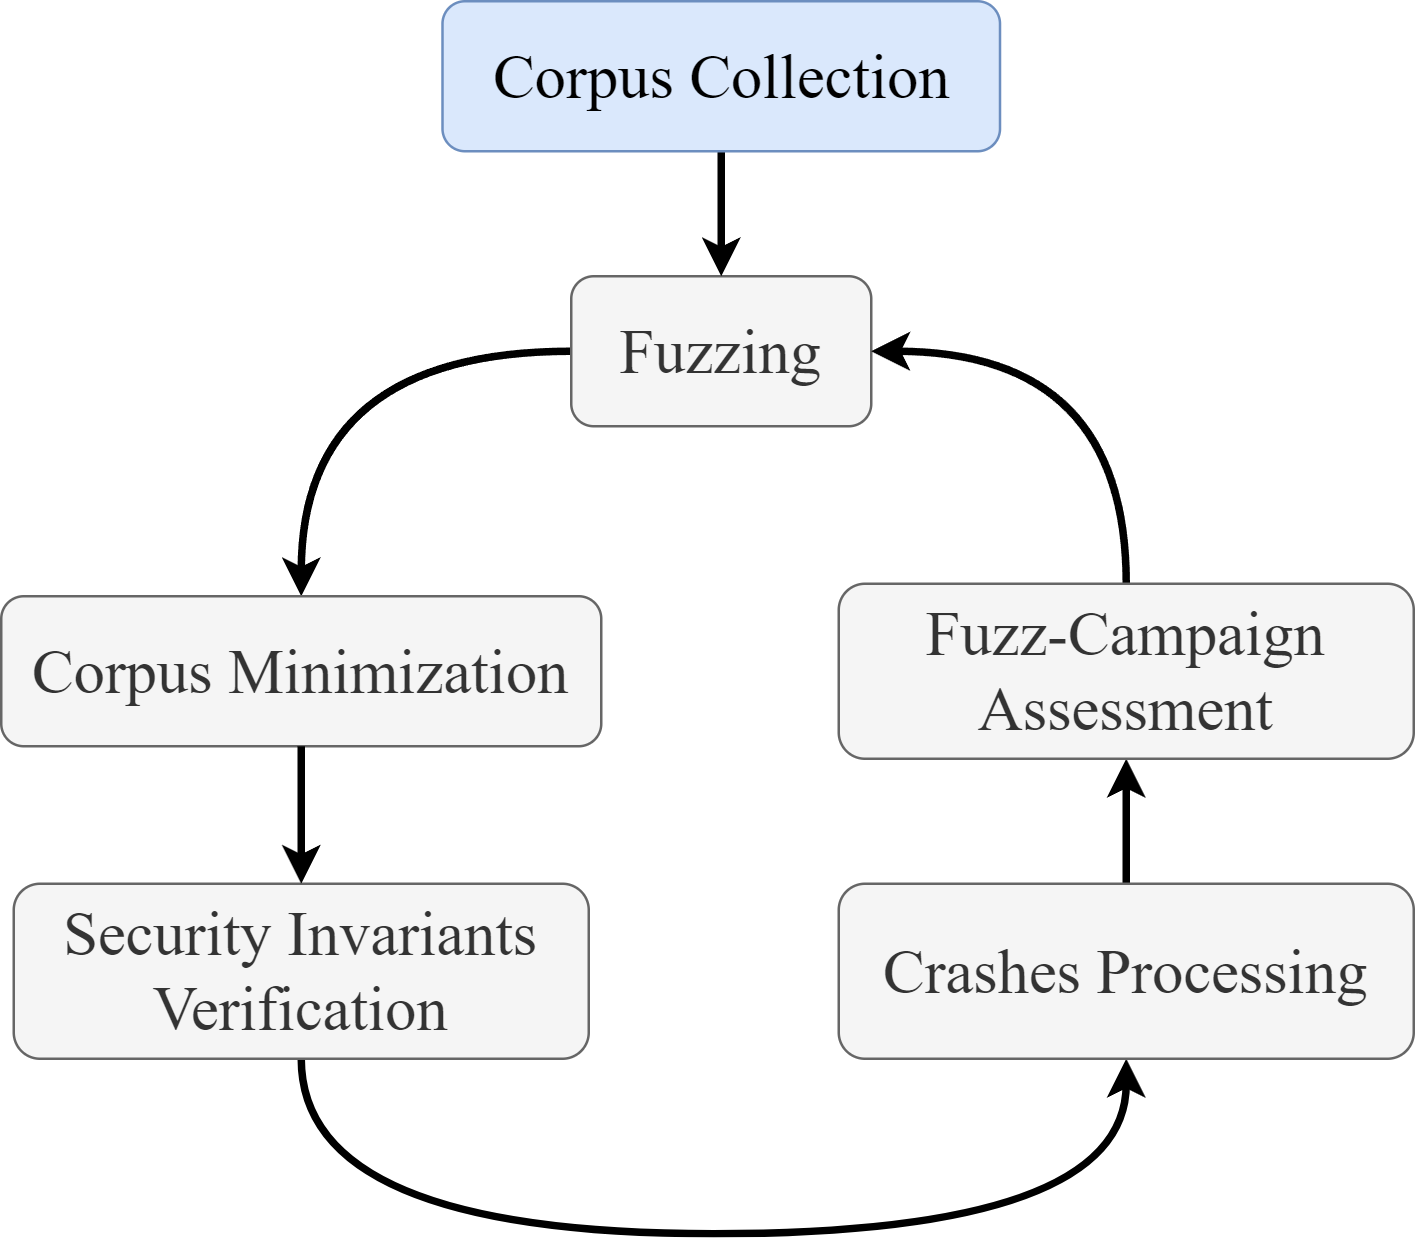
\includegraphics[width=10cm]{assets/dynamic-analysis-pipeline-tnr.png}
    \caption{Dynamic analysis pipeline}
    \label{fig:dynamic-analysis-pipeline}
\end{figure}

\newparagraph{Hybrid Fuzzing}

The first step of the pipeline is hybrid fuzzing. It is performed with the help of the \textit{sydr-fuzz} tool. The tool takes a toml configuration file as input, which contains the information about the fuzzing targets. The configuration file for the \texttt{jit\_differential} target is shown in Listing \ref{listing:jit-differential-config}.

\begin{listing}[h]
    \centering
    \begin{minipage}{.75\linewidth}
        \begin{minted}[linenos=true, tabsize=4, breaklines=true]{toml}
[sydr]
args = "-l debug"
target = "/jit_differential_sydr @@"

[libfuzzer]
path = "/jit_differential_fuzz"
args = "-detect_leaks=0 -rss_limit_mb=30720 -timeout=300 -report_slow_units=350 /ir_corpus"

[cov]
target = "/jit_differential_cov @@"
\end{minted}
    \end{minipage}
    \caption{Configuration file for the \texttt{jit\_differential} target}
    \label{listing:jit-differential-config}
\end{listing}

The configuration file contains three sections: \texttt{sydr}, \texttt{libfuzzer}, and \texttt{cov}. The \texttt{sydr} section contains information about the target program and how to execute it under the symbolic execution engine. The \texttt{libfuzzer} section contains libfuzzer-related information, such as the path to the fuzz target binary and the arguments that should be passed to it. Finally, the \texttt{cov} section contains information about the coverage target.

With the configuration file prepared, we can now start the fuzzing campaign. To do so, we need to execute the \textit{sydr-fuzz} binary as follows: \texttt{sydr-fuzz -c jit\_differential.toml run}. The command will start the fuzzing process and will print the results to the console.

\newparagraph{Corpus Minimization}

After running the fuzzer for some time, we can proceed to the next step of the pipeline - corpus minimization. The goal of this step is to reduce the size of the corpus by removing the redundant inputs. The corpus minimization is performed using the \textit{sydr-fuzz} tool in the \textit{cmin} mode.

This step is optional, however, it is highly recommended, because it greatly improves the performance of the next step - security invariants verification. Without corpus minimization, the security invariants verification is less likely to find any bugs, as it will potentially re-execute almost the same inputs multiple times.

\newparagraph{Security Invariants Verification}

The next step of the pipeline is security invariants verification. The idea behind this step is to execute the \textit{sydr} symbolic execution engine in the \textit{security} mode, with inputs from the minimized corpus. The \textit{security} mode is a special mode that is designed to check for violation of various security invariants, such as integer overflows, null pointer dereferences, buffer overflows, and others. If any of the invariants are violated, the symbolic execution engine will report the corresponding bug.

Running the symbolic execution engine in the \textit{security} mode is a very expensive operation. For this reason, we have worked on the optimization of this step. The results are discussed in chapter \ref{hybrid-fuzzer-improvements:optimizing-security-predicates}.

\newparagraph{Crashes Processing}

Near the end, we have the crashes processing stage. During previous steps, \textit{sydr-fuzz} may have found some crashes. At this stage, those crashes need to be processed. To do so, \textit{sydr-fuzz} employs the \textit{casr} tool \cite{casr-cluster-ispras-2021}. This tool performs automatic crashes processing, which includes deduplication, and clusterization.

Executing \textit{sydr-fuzz} in this mode, using the following command: \texttt{sydr-fuzz -c jit\_differential.toml casr}, will produce a set processed crashes.
\newparagraph{Fuzz-Campaign Assessment}

Finally, after all the steps are completed, we can assess the results of the fuzzing campaign. The assessment is performed manually by the user, and includes the following steps:

\begin{enumerate}
    \item Bug triaging and reporting
    \item Code coverage analysis
\end{enumerate}

During the bug triaging and reporting step, the user needs to analyze the found bugs and decide whether they are real bugs or not. If the bug is proven to be real, the user needs to report it to the developers of the target program.

The code coverage analysis step is performed to assess the effectiveness of the fuzzing campaign. The goal of this step is to help the user to understand whether the fuzzing campaign was effective and whether it is worth continuing it. The code coverage analysis is performed using the \textit{sydr-fuzz} tool in the \textit{cov} mode.

This concludes the description of the dynamic analysis pipeline, which has been used to fuzz the PyTorch framework. In the next section, we will discuss some of the findings.

\subsection{Results Overview}

As a result of our work multiple bugs were found in different parts of the PyTorch framework. Most of the bugs were found in the module responsible for unpickling, however we have also identified at least one remotely-accessible bug in the RPC module.

We have reported all the found bugs to the developers of the PyTorch framework. The developers have confirmed that all the bugs are real, and have merged the corresponding pull requests into the PyTorch repository. The pull requests are listed below:

\begin{itemize}
    \item \href{https://github.com/pytorch/pytorch/pull/94300}{\#94300: Add size check before calling stack\_.at(dict\_pos) in unpickler.cpp}
    \item \href{https://github.com/pytorch/pytorch/pull/94298}{\#94298: Add stack emptiness checks inside interpreter.cpp}
    \item \href{https://github.com/pytorch/pytorch/pull/94297}{\#94297: Add size check before calling .back() in rpc/script\_call.cpp}
    \item \href{https://github.com/pytorch/pytorch/pull/94295}{\#94295: Add exception handlers for stoll in schema\_type\_parser.cpp}
    \item \href{https://github.com/pytorch/pytorch/pull/91401}{\#91401: Add out-of-bounds checks inside irparser.cpp and unpickler.cpp}
\end{itemize}

In section \ref{results:pytorch-bugs}, we will take a closer look at the bugs we found and the pull requests we created.
